\chapter{Project Plan} \label{Project-Plan}

\lhead{Chapter 5. \emph{Project Plan}}

The project development will start from the 2nd of May and end on the 15th of August. We will discuss the multiples steps of this project and how these steps are planned. You can find the Grant chart summing things up in figure \ref{fig:gantt-chart}.

Here are the multiple steps:
\begin{enumerate}
    \item \textbf{Implement a flexible environment}: To train my neural network and test it I will need to have a flexible game interface with which I can easily play/reset the game, go some steps backs, etc. Besides, this environment interface should aim to be universal to any imperfect games. Given so it will be easy to change from one game to another. I may also re-use some work on this, for example, rlcard \citep{zha2019rlcard}.
    \item \textbf{Implement Kuhn poker interface}: This will require searching the equilibrium of Kuhn poker. This will be the first game on which we will start working.
    \item \textbf{Implement evaluation/teaching agents for Kuhn poker}: implement of the different kind of agents presented in section \ref{subsection:evaluation}. As you can see in the gantt chart \ref{fig:gantt-chart}, this task is split into two iterations, it is because at first, only some agents will be necessary to evaluate and train the NN. Then while improving the NN more sophisticated agents would need to be implemented.
    \item \textbf{Implement the neural networks}: implementation of the opponent modelling NN (section: \ref{methodology:opponent-modelling}) and the decision making NN (section: \ref{methodology:opponent-modelling}).
    \item \textbf{Implement the EA training}: As described in section \ref{methodology:competitive-co-evolution}, implementation of the EA with competitive co-evolution.
    \item \textbf{Implement the reinforcement learning}: This step is optional if EA training have good performance.
    \item \textbf{Test the NN}: more information in section \ref{subsection:evaluation}
    \item \textbf{Scale up the algorithm} to a game with a larger game state.
    \begin{enumerate}
        \item \textbf{Implement an other game interface}
        \item \textbf{Manage the equilibrium approximation}: game with a large game tree such as poker texas holdem do not have a pre-computed equilibrium because the game tree is too large. We will need to use an equilibrium approximation. 
        \item \textbf{Create / Use game abstraction}: this task is optional but will likely be required to reduce the info set size and action set size.
        \item \textbf{Troubleshoot scale up issue}: We can not write a detailed description because we do not know which part will have scalability issue. In addition the time estimation in the gantt chart (figure: \ref{fig:gantt-chart}) is just a wild estimation and can vary a lot. It is worth to mention that the time hazard of this task has been taken in consideration, refer section \ref{subsection:risk-assesment} for more details.
    \end{enumerate}
    \item \textbf{Write the dissertation}
\end{enumerate}

\begin{figure}[ht]
    \centering
    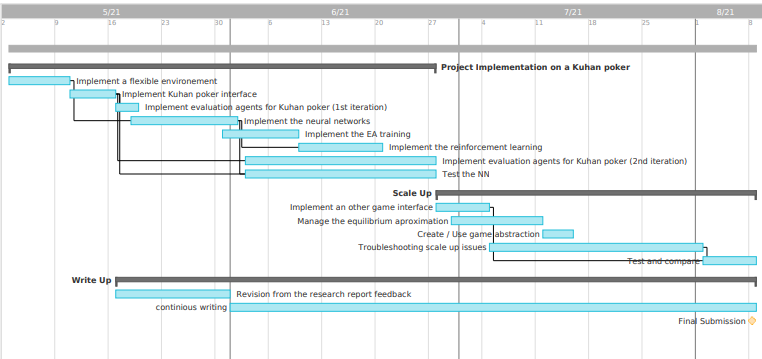
\includegraphics[width=1\textwidth]{Figures/gantt-chart.png}
    \caption{Gantt Chart}
    \label{fig:gantt-chart}
\end{figure}